% =====================================================================
% Considerações finais — Esboço de seção (análise de rede textual da
% TESE INTEIRA). Primeira camada (co-ocorrência + Louvain) aplicada ao
% corpus completo, no mesmo molde das figuras dos capítulos 1 a 4, mas
% sobre a tese toda de uma vez. É o mesmo grafo que a capa do site
% renderiza de forma interativa (tese_network.py); aqui ele entra como
% inscrição estática que fecha o argumento.
%
% Estilo seguido (regras da tese): primeira pessoa do singular, sem
% travessões em texto principal, "capítulo" minúsculo, aspas com
% \enquote{}, sem fórmulas do tipo "não X, mas Y".
%
% Observação técnica: a figura é gerada por
%   infranodus/render_tese_network_figura.py  ->  figuras/rede_tese_inteira.png
% =====================================================================

\subsection*{A tese inteira como uma rede: uma inscrição final}

Ao encerrar, aplico à tese inteira o procedimento de análise de rede
textual que introduzi no capítulo~\ref{capitulo1} e mobilizei capítulo a
capítulo, agora sobre o corpus completo de uma vez, da Apresentação às
Considerações finais. É o mesmo grafo que o site renderiza de forma
navegável, congelado aqui em uma inscrição estática que me deixa ver a
arquitetura conceitual do trabalho como um todo. O grafo reúne os 260
termos de maior frequência da tese e detecta, por Louvain, sete
comunidades que reconheço, uma a uma, como as regiões do meu próprio
argumento: a etnografia e o método, o projeto SPIRA, o arranjo do C4AI, as
figurações e a genealogia militar, a inteligência artificial como objeto,
a teoria ator-rede e o panorama bibliométrico do campo.

O centro absoluto do grafo é \textit{rede}, com o maior \textit{degree}
(4.095) e a maior \textit{betweenness} (0,36) de toda a tese. A palavra
condensa a ambivalência que percorre o trabalho, já que nela se encontram
a rede sociotécnica que descrevo e a análise de rede que pratico, e é por
ela que transita a maior parte do vocabulário. Ao seu redor, os termos de
maior centralidade desenham a espinha da tese: \textit{artificial},
\textit{inteligência}, \textit{pesquisa}, \textit{spira}, \textit{ciência},
\textit{latour}, \textit{dado} e \textit{objeto}. As maiores pontes por
\textit{betweenness}, além de \textit{rede}, são \textit{spira} (0,18),
\textit{pesquisa} (0,16), \textit{ciência} (0,15) e \textit{latour}
(0,15), com \textit{inscrição} comparecendo logo em seguida (0,06): os
termos que costuram os capítulos entre si são, ao mesmo tempo, o objeto
empírico (SPIRA), o campo (pesquisa, ciência), o interlocutor teórico
(Latour) e o conceito que atravessa a tese toda (a inscrição).

\begin{figure}[!htb]
\centering
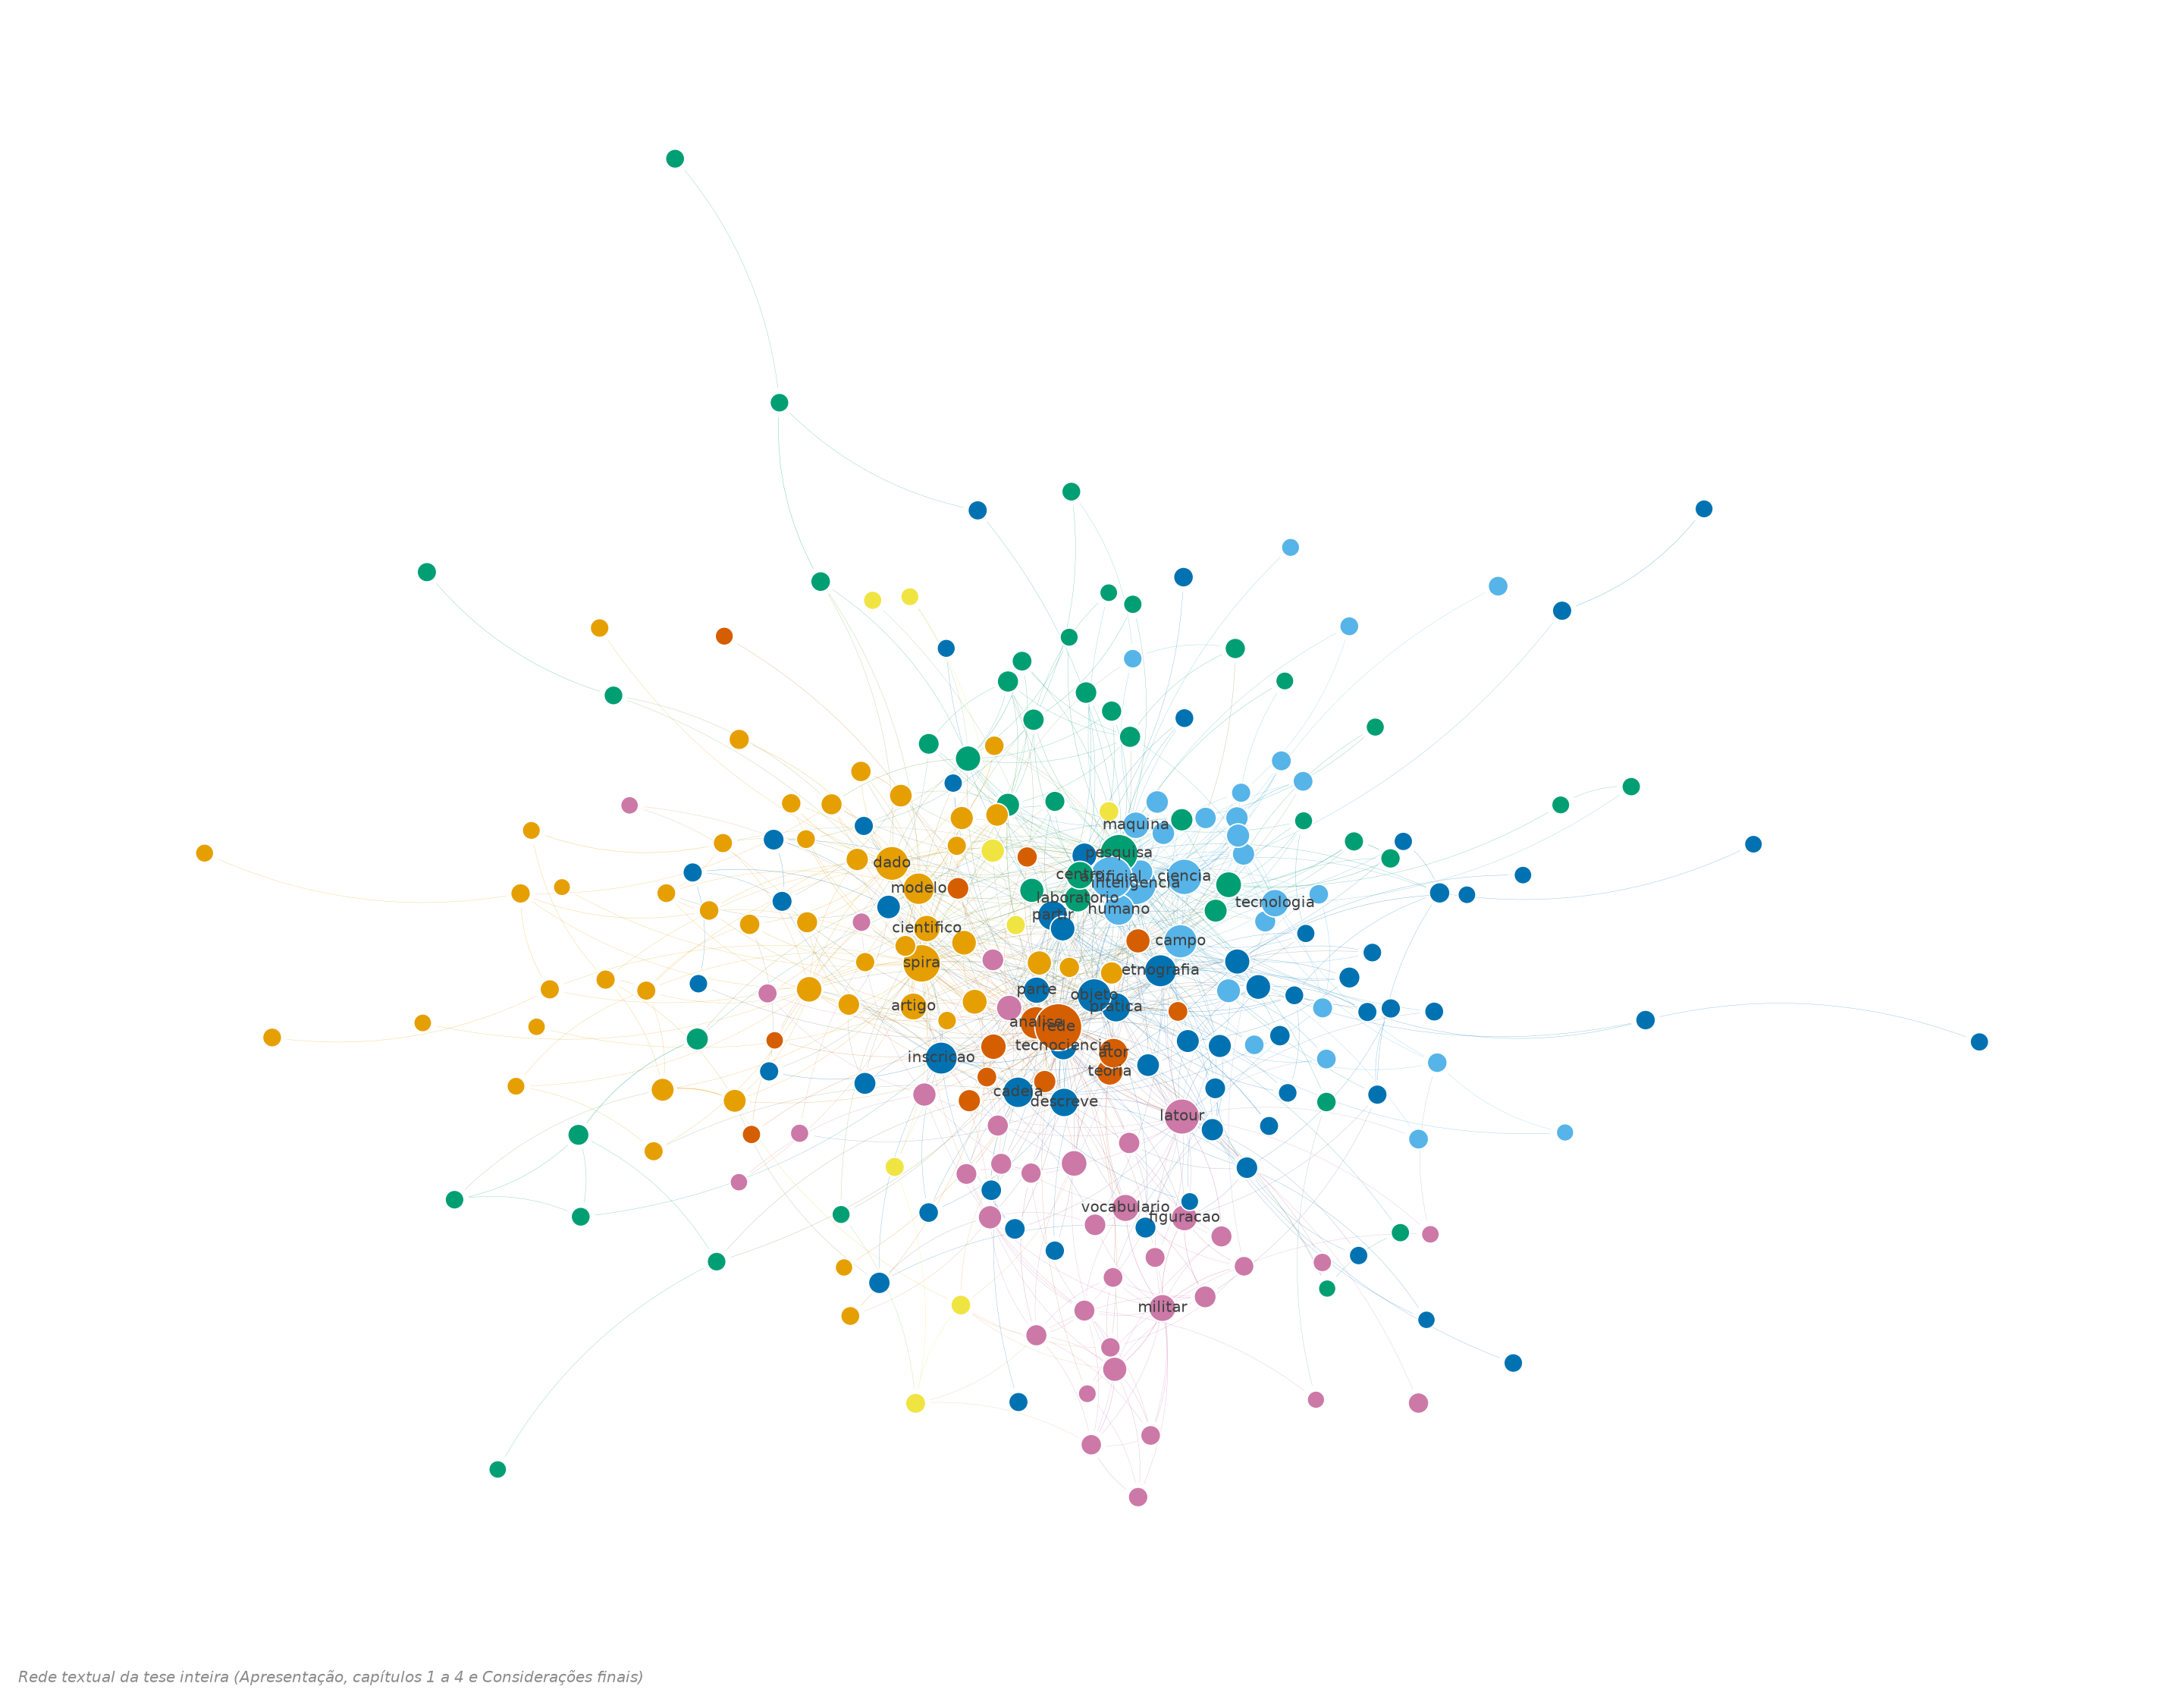
\includegraphics[width=1.0\textwidth,keepaspectratio]{figuras/rede_tese_inteira.png}
\caption[Rede textual da tese inteira (\textit{text network
analysis})]{Rede textual da tese inteira, da Apresentação às
Considerações finais (\textit{text network analysis}). Os nós são os
termos de maior \textit{degree} ponderado, com o tamanho proporcional ao
\textit{degree}; a cor indica a comunidade detectada por Louvain
ponderado sobre o corpus completo; as arestas, arqueadas, recebem a
mistura das cores das comunidades que ligam. Por legibilidade, a versão
impressa retém as co-ocorrências de peso mais alto; a versão navegável,
com todas as ligações, está no site que acompanha esta tese. Arquivo de
alta resolução e dados em \texttt{infranodus/} no repositório.}
\label{fig:infranodus-tese}
\end{figure}

As co-ocorrências de maior associação (NPMI) funcionam como um índice dos
compromissos conceituais que sustento de ponta a ponta. A cena clínica do
SPIRA aparece na dupla mais forte de toda a tese,
\textit{respiratória}~$\leftrightarrow$~\textit{insuficiência} (0,87); o
objeto técnico se fixa em \textit{inteligência}~$\leftrightarrow$~%
\textit{artificial} (0,85) e em \textit{máquina}~$\leftrightarrow$~%
\textit{aprendizado} (0,63); o campo etnográfico deixa seus atores em
\textit{cláudio}~$\leftrightarrow$~\textit{fábio} (0,69) e
\textit{engenheiro}~$\leftrightarrow$~\textit{cientista} (0,74); o aparato
teórico se condensa em \textit{teoria}~$\leftrightarrow$~\textit{ator}
(0,68) e \textit{mediação}~$\leftrightarrow$~\textit{técnica} (0,61); e a
genealogia militar-industrial do capítulo~\ref{capitulo2} sobrevive no
todo pelos pares \textit{indústria}~$\leftrightarrow$~\textit{militar}
(0,59) e \textit{rótulo}~$\leftrightarrow$~\textit{militar} (0,57). Lida
pela sua própria rede, a tese se mostra amarrada por poucos pares densos,
um por região do argumento, e por um vocabulário genérico que faz a
ligação entre eles.

Duas leituras fecham este gesto. A primeira é que a partição da tese
inteira recupera a estrutura dos capítulos sob a forma de comunidades, o
que me diz que os capítulos deixaram marca lexical própria e legível, e
que a costura entre eles se faz por um núcleo compacto de termos
ator-rede: a comunidade da teoria ator-rede é a menor em tamanho (quinze
termos: \textit{rede}, \textit{análise}, \textit{ator}, \textit{teoria},
\textit{actante}), e ainda assim a mais central e a que mais faz ponte, ao
passo que os objetos empíricos (SPIRA, C4AI, a inteligência artificial)
ocupam as comunidades maiores. A tese se sustenta, portanto, por um
vocabulário de método enxuto que atravessa territórios empíricos amplos. A
segunda leitura é reflexiva e retoma o gesto que abre o capítulo~%
\ref{capitulo1}: submeter a tese ao tratamento que ela dá aos seus objetos
produz uma última inscrição, o móvel imutável do argumento inteiro, e
reconhecer que a análise mede o que também ajuda a produzir é a forma mais
honesta de encerrar um trabalho que se propôs a descrever a tecnociência
sem apagar a técnica que o sustenta.
